\section{Experimental Setup}
\subsection{Evaluation Metrics}
Models were evaluated on 10,027 hold-out test sequence windows using multi-class metrics: Accuracy, One-vs-Rest (OvR) Macro Precision, Macro Recall, Macro F1-score, Weighted F1-score, Macro Area Under the Receiver Operating Characteristic Curve (ROC-AUC), and Macro Area Under the Precision-Recall Curve (PR-AUC).

\subsection{Hyperparameter Settings \& Training Protocol}
Global random seed \texttt{SEED = 42} was enforced across PyTorch, NumPy, and Scikit-Learn to guarantee experiment reproducibility. Models were trained using \texttt{optim.Adam} ($lr = 0.001$, weight decay $10^{-5}$) and multi-class \texttt{nn.CrossEntropyLoss()} for 50 epochs with a batch size of 64. Early stopping with a patience of 10 epochs monitored validation loss.

Fig. \ref{fig:loss_curves} illustrates training and validation loss trajectories for Informer vs. GRU over 50 epochs. While GRU exhibits validation loss divergence after epoch 20 due to spatial-temporal overfitting, Informer demonstrates smooth, non-divergent loss convergence across all 50 epochs. Deployed checkpoint \texttt{epoch\_10.pth} was saved for production backend serving.

\begin{figure}[htbp]
\centering
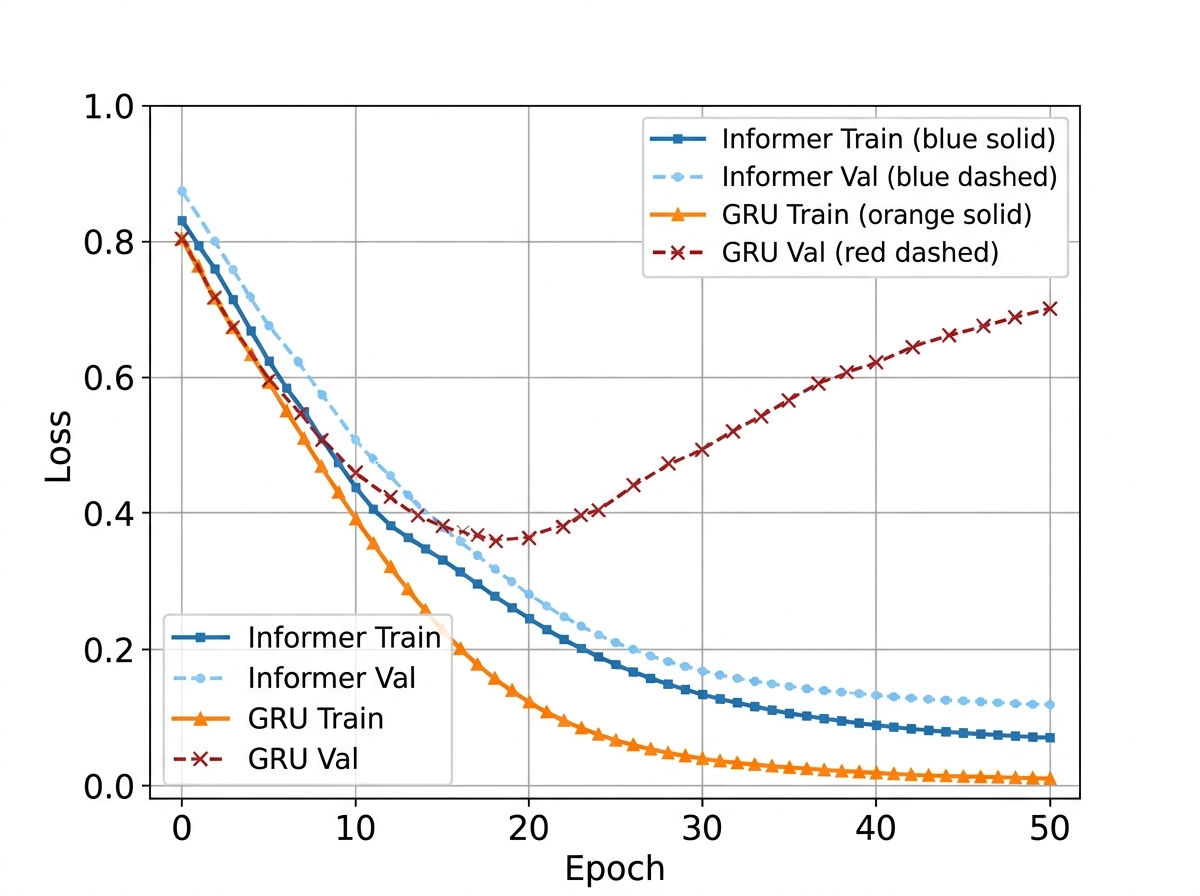
\includegraphics[width=0.88\linewidth]{figures/fig2_informer_loss.jpg}
\caption{Informer vs. GRU Training and Validation Loss Curves Across 50 Epochs.}
\label{fig:loss_curves}
\end{figure}

\subsection{Hardware and Software Specifications}
All model training and benchmarking were executed on a Windows workstation equipped with an Intel Core i7 processor, 32 GB RAM, and an NVIDIA GeForce RTX GPU. Experiments were implemented in Python 3.10 using PyTorch 2.1, Scikit-Learn 1.3, and FastAPI 0.104.
